\documentclass[a4paper]{article}

\usepackage{amsmath,amssymb,amsthm,thmtools,thm-restate,bbm,cancel,hyperref,graphicx}
\newcommand{\lc}{\left\{}
\newcommand{\rc}{\right\}}
\renewcommand{\notin}{\not\in}
\renewcommand{\epsilon}{\varepsilon}
\newcommand{\E}{\mathbb{E}}
\newcommand{\I}{\mathbbm{1}}
\newcommand{\N}{\mathbbm{N}}
\newcommand{\Sum}{\sum\limits_{i=1}^N}
\newcommand{\qedsquare}{\tag*{$\square$}}
\newcommand{\fn}{\frac{1}{N}}
\newcommand{\mn}{\frac{m}{N}}
\newcommand{\de}{\delta^{-1}e^{-\mn}}
\newcommand{\e}{e^{-1.0051 \mn}}
\newcommand{\df}{\delta^{-1}(1-\e)}
\newcommand{\odf}{1-\delta^{-1}(1-\e)}

\title{Assignment 1}
\author{
    Ory Band \texttt{300479425} \and
    Uri Menkes \texttt{300691367}}
\date{\today}

\newtheorem{thm}{Theorem}

\usepackage{fancyhdr}
\pagestyle{fancy}
\lhead{Ory Band \texttt{300479425}, Uri Menkes \texttt{300691367}}
\rhead{}
\renewcommand{\headrulewidth}{0.4pt}
\renewcommand{\footrulewidth}{0.4pt}

\begin{document}

\maketitle
\newpage

\section {Question 1}
\subsection {(a)}

First, we'll notice that we're discussing discrete distributions (and not absoloutly continuous ones, for example).
Therefore, since $ \forall 1 \leq i \leq N : X_i \sim P $, we get that $ \Pr(x_i=i)=p_i $.

According to the description,
$ \forall 1 \leq i \leq N : \Pr(i \in A) = p_i \cdot \I_{ \lc X_1 \neq i \wedge X_2 \neq i \wedge .. \wedge X_m\neq i \rc }   $. \\
Therefore, using the \textit{linearity of expectation}, we can write:
\begin{align*}
    \E[U_m] = \E \Bigg[ \Sum p_i \cdot \I_{ \lc X_1 \neq i \wedge X_2 \neq i \wedge .. \wedge X_m\neq i \rc } \Bigg]
    &= \Sum p_i \cdot \E \Big[ \I_{\lc..\rc} \Big] \\
\end{align*}
And since $ X_1, X_2, .., X_m $ are \textit{independent}, and $ (1-p_i)^m $ is constant, we get:
\begin{align*}
    &= \Sum p_i \cdot \E \Big[ \I_{\lc X_1 \neq i \rc} \cdot \I_{\lc X_2 \neq i \rc}, .. , \I_{\lc X_m \neq i \rc} \Big] \\
    &= \Sum p_i \cdot \E \Big[ \I_{\lc X_1 \neq i \rc} \Big] \cdot \E \Big[ \I_{\lc X_2 \neq i \rc} \Big] \cdot .. \cdot \Big[ \I_{\lc X_m \neq i \rc} \Big] \\
    &= \Sum p_i \cdot (1-p_i)^m \\
    \qedsquare
\end{align*}

\newpage

\subsection {(b)}

\subsubsection {First sub-question}

Notice that $ \forall x \in \mathbb{R} : 1-x \leq e^{-x} $ . Therefore:
\begin{align*}
    \E[U_m] = \Sum \fn \cdot \Big( 1-\fn \Big)^m = \cancel{N} \cdot \cancel{\fn} \cdot \Big(1-\fn \Big)^m \leq (e^{-\fn})^m = e^{-\mn}
\end{align*}

\subsubsection {Second sub-question}
Notice that $ \E[U_m] = \Big(1-\frac{1}{N}\Big)^m \geq \e \iff
\Big(1-\frac{1}{N}\Big)^N \geq e^{-1.0051} $. \\
For $ N = 100 $, it is true that $ (1-\frac{1}{100})^{100} \approx 0.36603
\geq 0.36600 \approx e^{\frac{-1.0051}{100}} $. \\

Denote the function $ f(x)=(1-\frac{1}{x})^x $, \\
Calculating the derivative gives us $ f'(x) = (1-\frac{1}{x})^x \cdot \Big[ \ln(1-\frac{1}{x}) + \frac{1}{x-1} \Big] $ \\
What is left to ask if for which $x$ it is true s.t. $ f'(x) > 0 $ ? Notice that:
\begin{align*}
    \forall x > 100 :
    (1-\frac{1}{x})^x &> 0, \\
    \ln(1-\frac{1}{x}) &< 0, \\
    \frac{1}{1-x} &> 0, \\
    |\frac{1}{x-1}| &> |\ln(1-\frac{1}{x})| \\
    \\
    \Rightarrow f'(x) &> 0 .
\end{align*}
From this we can decuce that if $ (1-\frac{1}{100})^{100} \geq e^{-1.0051} $, \\
then $ \forall N \geq 100 : \Big( 1-\fn \Big) ^N \geq e^{-1.0051} $.

This proves that $ \Big( 1-\fn \Big)^m = \E[U_m] \geq \e $.

\subsubsection {Third sub-question}

Let $ 0 < \delta < 1 $, and notice $ U_m \geq 0 $ is a simple random variable, because $ N \subseteq \N $. \\
From \textit{Markov's inequality} and the previous sub-question we get:
\begin{align*}
    \Pr \Big( U_m \geq \delta^{-1} e^{\mn} \Big) &\leq \frac{\E[U_m]}{\de}
    \leq \frac{\cancel{e^{\mn}}}{\delta^{-1}{\cancel{e^{-\mn}}}} = \frac{1}{\delta^{-1}} = \delta \\
    \Rightarrow \Pr \Big( U_m < \de \Big) &= 1 - \Pr \Big( U_m \geq \de \Big) \geq 1-\delta \\
    \qedsquare
\end{align*}

\newpage

\subsubsection {Fourth sub-question}

\begin{align*}
    \Pr( U_m \geq \odf)
    &= \Pr( 1 - U_m \leq \df ) \\
    &= 1 - \Pr( 1 - U_m > \df ) \\
    &\geq 1 - \frac{\E[1-U_m]}{\df} && (Markov's\ inequality) \\
    &\geq 1 - \frac{1-\e}{\df} && (N \geq 100) \\
    &= 1 - \delta
    \qedsquare
\end{align*}

\subsubsection {Fifth sub-question}

Now, from the previous quesion, for $ m = \frac{ N \ln \frac{25}{9} }{1.0051} \approx 1.017 N $ and for $ \delta=\frac{4}{5} $ we get: \\
\begin{align*}
    \Pr \Big( U_m \geq 1 - \frac{5}{4} ( 1 - e^{ - \cancel{1.0051}
        \frac{ \cancel{N} \ln \frac{25}{9} }{\cancel{1.0051} \cancel{N}}} ) \Big)
    &= \Pr \Big( U_m \geq 1 - \frac{5}{4} ( 1 - e^{ - \ln \frac{25}{9} } ) \Big) \\
    &= \Pr \Big( U_m \geq 1 - \frac{5}{4} ( 1 - \frac{9}{25} ) \Big) \\
    &= \Pr \Big( U_m \geq \frac{1}{5} \Big) && (Previous\ sub-question) \\
    &\geq 1 - \frac{4}{5} \\
    &= \frac{1}{5}
\end{align*}
And for $m < \frac{ N \ln \frac{25}{9} }{1.0051} $ the inequality still holds (the right wing inside $\Pr$ gets smaller).
\begin{align*}
    \qedsquare
\end{align*}

\newpage

\subsection {(c)}

\subsubsection {First sub-question}

We need to show that $ \forall \epsilon , \delta > 0 : \Pr ( |U_m| > \epsilon ) \xrightarrow{m \to \infty} 0 $

Notice that $ U_m \geq 0 $ thus $ |U_m| = U_m $, and that for $ N=\N , P = { p_1, p_2, .. } $ \\
we have $ \displaystyle \lim_{N \to \infty} \Sum p_i = 1 $ because $ P(\N) = 1 $. \\
Furthermore, $ \forall i \in N : 0 \leq p_i \leq 1 $ thus $ (1-p_i)^m \xrightarrow{m \to \infty} 0 $. \\
Therefore from \textit{Markov's inequality} and \textit{(a)} we get:
\begin{align*}
    \Pr ( |U_m| > \epsilon ) = \Pr ( U_m > \epsilon ) &\leq \frac{\E[U_m]}{\epsilon} \\
    &= \frac{ \Sum p_i ( 1 - p_i ) ^m }{\epsilon} \\
    &= \frac{ \Sum p_i ( 1 - p_i ) ^m }{\epsilon} \\
    &<_{m \to \infty} \frac{ \Sum p_i \cdot \epsilon \cdot \delta }{\epsilon} \\
    &= \frac{ \cancel{\epsilon} \cdot \delta }{\cancel{\epsilon}} \cdot \Sum p_i \xrightarrow{N \to \infty} \delta
    \qedsquare
\end{align*}

\subsubsection {Second sub-question}

First lets stand on the difference between PAC and CAP:
\begin{align*}
    &PAC: \forall \epsilon , \delta > 0 : \exists m_0 : \forall P, c\in\mathcal{C}, m>m_0 : \Pr( err(h) > \epsilon ) <\delta \\
    &CAP: \forall \epsilon , \delta > 0 : \forall P, c\in\mathcal{C} : \exists m_0 :\forall m>m_0 : \Pr( err(h) > \epsilon ) <\delta
\end{align*}

Denote at the following problem: $ \mathcal{X}=\N, \mathcal{C}= \lc 0,1 \rc^{\N} $ \\
We need to show that for any given $ c \in \mathcal{C} $, the problem is CAP-learnable but not PAC-learnable.

In the previous sub-question we showed that for every $ \epsilon, \delta > 0 $ and for every $P$ over $\N$,
there is $ m_0(\epsilon,\delta) $ s.t. for every $ m > m_0 $ we have $ \Pr(U_m > \epsilon) < \delta $. \\
This exactly means that the given problem is CAP-learnable.

However, from question \textbf{(b)}, and for $ \epsilon := \frac{1}{5}, \delta := \frac{1}{6} $ and for the uniform distribution
(like in \textbf{(b)}), but over $\N$ instead of any finite $[N]$, and for any $ c \in \mathcal{C} $,
we have that for every $m_0$ there exists a $m$ s.t. $m>m_0$ and we have:
$ \Pr(U_m \geq \frac{1}{5}) \geq \frac{1}{5} > \frac{1}{6} $.
This means that the problem is \textbf{not} PAC-learnable.
\begin{align*}\qedsquare\end{align*}

\newpage

\section {Question 2}

We think Simplicio is wrong:

\begin{enumerate}
    \item Notice that Simplicio's analysis model is not a PAC anaylsis:
        \begin{align*}
            &PAC: \forall \epsilon , \delta > 0 : \exists m_0 : \forall P, c\in\mathcal{C}, m>m_0
            : \Pr( err(h) > \epsilon ) <\delta \\
            &Simplicio: \forall D, R, m_0 : \exists \epsilon : \Pr( err(h) > \epsilon ) \geq 1 - e^{m\epsilon}
        \end{align*}

    \item The distribution $D$ and square $R$ aren't known in a PAC problem -
        only the $m$ samples and $\epsilon,\delta$ are known.
        Simplicio makes $\epsilon$ dependent upon the \textit{given distribution and square} $D,R$, and not the other way around.

    \item Likewise, the number of required samples $m_0$ is not dependent upon $D,R$.
\end{enumerate}

\section {Question 3}

\subsection {(a)}

The \textit{reverse Markov inequality} gives a lower bound: \\
\url{http://planetmath.org/reversemarkovinequality}
\begin{restatable}[Reverse Markov Inequality]{thm}{markov}
    \label{thm:markov}
    Let $X$ be a random variable that satisfies $ \Pr(X \leq a) = 1 $ for some constant $a$.
    Then, for $ d < E[X] $:
    \begin{align*}
        \Pr(X>d) \geq \frac{\E[X] - d}{a - d}
    \end{align*}
\end{restatable}
\begin{proof}
    Let $Y:=a-X$ and apply the original Markov inequality:
    \begin{align*}
        &\Pr(X\leq d) = \Pr(Y\geq a-d) 
        \leq \frac{\E[Y]}{a-d} 
        = \frac{a-\E[X]}{a-d} \\
        \Rightarrow &\Pr(X>d) \geq 1 - \frac{a-\E[X]}{a-d} = \frac{\E[X]-d}{a-d}
    \end{align*}
\end{proof}

For the lower bound to be non-trivial, we require: $t<\E[X]$ \\
and $ a\in\mathbb{R} : \Pr(x \leq a) = 1 $

\subsection {(b)}

Let $(X_n)_{n=1}^{\infty}$ be a series of random variables, s.t.:\\
\begin{align*}
    \forall n: X_n (s) := \lc
    \begin{array}{ll}
        \frac{1}{n} & \mbox{$s=n$} \\
        0 & \mbox{otherwise}
    \end{array} \right.
    \Rightarrow \E[X_n] = \cancel{n} \cdot \frac{1}{\cancel{n}} + \cancel{0 \cdot (1 - \frac{1}{n})} = 1 \\
\end{align*}
Any by \textit{Markov's inequality} we get: $ \Pr(X_n \geq n) \leq \displaystyle \frac{\E[X_n]}{n} = \frac{1}{n} $ \\
But according to the definition of $X_n$ we actually have $\Pr(X_n>n)=0$ therefore getting $\Pr(X_n>n)=\frac{1}{n}$ \\
\begin{align*}\qedsquare\end{align*}

\subsection {(c)}

This is \textit{Paley-Zigmund inequality}. For the proof we need a helper-theorem:

\begin{restatable}[Law of Total Expectation]{thm}{total}
    \label{thm:total}
    Let $X$ be a random variable s.t. $|\E[X]|<\infty$ and let $Y$ be any random variable on the same probabilty space.
    Then:
    \begin{align*}
        \E[X] = \E_Y \Big[ \E_{X|Y} [X|Y] \Big]
    \end{align*}
\end{restatable}

Now for solving our question. First notice:

\begin{align*}
    \E[X \cdot \I_{\lc..\rc}] &= \E \Bigg[ \E \Big[ X \cdot \I | X < t \cdot \E[X] \Big] \Bigg] \\
    &= \E \Big[ \E [ X | X < t \cdot \E[X] ] \Big] && (X<t \cdot \E[X]) \\
    &\leq \E \Bigg[ \E \Big[ t\cdot\E[X] | X < t \cdot \E[X] \Big] \Bigg] && (X<t\cdot\E[X]) \\
    &= t\cdot\E[X] && (t\cdot\E[X]\ is\ constant)
\end{align*}

Thus we get:

\begin{align*}
    \E[X] &= \E \Big[ X \cdot \I_{\lc X < t \cdot \E[X] \rc} + X \cdot \I_{ \lc X \geq t \cdot \E[X] \rc } \Big] \\
    &= \E[X\cdot\I_{<}] + \E[X\cdot\I_{\geq}] \\
    &\leq t\cdot\E[X] + \sqrt{ \E[X^2] \cdot \E[\I_{\geq}] } && (Previous\ paragraph) \\
\end{align*}
\begin{align*}
    &\iff \E[X] - t\cdot\E[X] \leq \sqrt{E[X^2]} \cdot \sqrt{\E[\I]} \\
    &\iff (1-t) \cdot \E[X] \leq \sqrt{E[X^2]} \cdot \sqrt{\E[\I]}  \\
    &\iff (1-t)^2 \cdot \frac{(\E[X])^2}{E[X]} \leq \E[ \I_{ \lc X \leq \cdot \E[X] \rc} ]
    = Pr( X \geq t \cdot \E[X] )
    \qedsquare
\end{align*}

\newpage

\section {Question 4}

We used a simple average over the samples for approximating the biased coin parameter $p$.
According to the \textit{law of large numbers}, we have:
\begin{align*}
    \displaystyle \Pr \Bigg( \lim_{N \to \infty} | \Big( \frac{1}{N} \Sum X_i \Big) - p | > \epsilon \Bigg) = 0
\end{align*}
This explains the "downslope" curve of the error towards zero:

\begin{figure}[h!]
    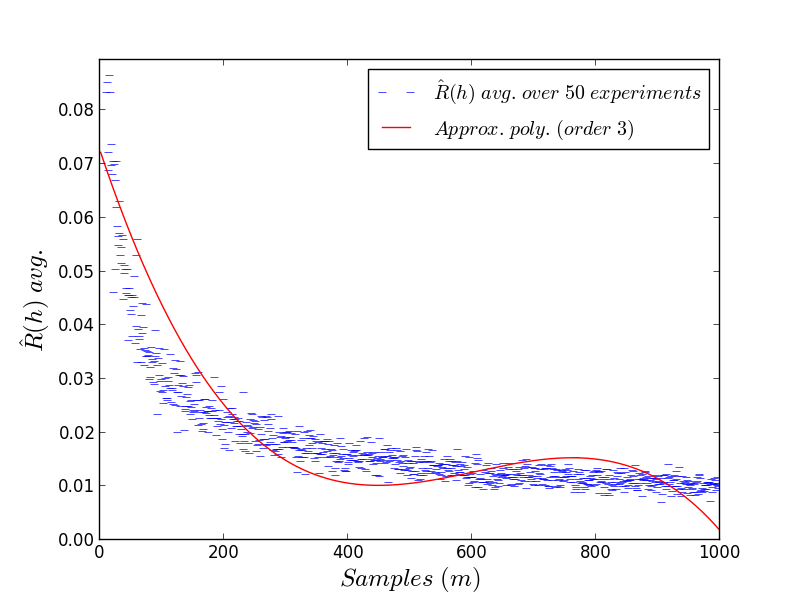
\includegraphics[width=0.9\textwidth]{q4.png}
    \caption{Code is at \url{https://github.com/oryband/machine-learning/blob/master/ass1/q4.py}}
\end{figure}

\begin{align*}\qedsquare\end{align*}

\end{document}
